\documentclass[a4paper,10pt,ngerman]{scrartcl}
\usepackage{babel}
\usepackage[T1]{fontenc}
\usepackage[utf8x]{inputenc}
\usepackage[a4paper,margin=2.5cm,footskip=0.5cm]{geometry}
\usepackage{wrapfig}
%\usepackage[english]{babel} 


% Die nächsten vier Felder bitte anpassen:
\newcommand{\Aufgabe}{Aufgabe 4: Würfelglück } % Aufgabennummer und Aufgabennamen angeben
\newcommand{\TeamId}{?????}                       % Team-ID aus dem PMS angeben
\newcommand{\TeamName}{234bcd}                 % Team-Namen angeben
\newcommand{\Namen}{Michael Köhler}           % Namen der Bearbeiter/-innen dieser Aufgabe angeben
 
% Kopf- und Fußzeilen
\usepackage{scrlayer-scrpage, lastpage}
\setkomafont{pageheadfoot}{\large\textrm}
\lohead{\Aufgabe}
\rohead{Team-ID: \TeamId}
\cfoot*{\thepage{}/\pageref{LastPage}}

% Position des Titels
\usepackage{titling}
\setlength{\droptitle}{-1.0cm}

% Für mathematische Befehle und Symbole
\usepackage{amsmath}
\usepackage{amssymb}

% Für Bilder
\usepackage{graphicx}
\graphicspath{ {./images/} }

% Für Algorithmen
%\usepackage{algpseudocode}

% Für Quelltext

\usepackage{listings}
\usepackage{color}
\definecolor{mygreen}{rgb}{0,0.6,0}
\definecolor{mygray}{rgb}{0.5,0.5,0.5}
\definecolor{mymauve}{rgb}{0.58,0,0.82}
 \definecolor{cloudwhite}{rgb}{0.225, 0.225, 0.204} 
\definecolor{red}{rgb}{0.4,0,0} 
\definecolor{blue}{rgb}{0,0,0.6}
\definecolor{green}{rgb}{0,0.6,0}
\definecolor{cyan}{rgb}{0.0,0.6,0.6}
\lstset{
language=csh,
basicstyle=\footnotesize\ttfamily,
numbers=left,
numberstyle=\tiny,
numbersep=5pt,
tabsize=2,
extendedchars=true,
breaklines=true,
frame=tb,
showspaces=false,
showtabs=false,
xleftmargin=17pt,
framexleftmargin=17pt,
framexrightmargin=5pt,
framexbottommargin=4pt,
showstringspaces=false,
% confing for comments
commentstyle=\color{green},
morecomment=[l]{//}, 
morecomment=[s]{/*}{*/}, 
% keywords for classes
morekeywords={  List, Program,GameResult,MatchUp,Player,Random },
keywordstyle=\color{cyan},
identifierstyle=\color{cloudwhite},
% keywords for types
emph={int,char,double,float,unsigned,void,bool,var,string,private,static,new,class,using},
emphstyle={\color{blue}},
% other keywords to highlight
classoffset=1, 
otherkeywords={throw,return,break},
morekeywords={throw,return,break},
keywordstyle=\color{mymauve},
classoffset=0,
% style for strings
stringstyle=\color{red}\ttfamily,
}


% Diese beiden Pakete müssen zuletzt geladen werden
%\usepackage{hyperref} % Anklickbare Links im Dokument
\usepackage{cleveref}

% Daten für die Titelseite
\title{\textbf{\Huge\Aufgabe}}
\author{\LARGE Team-ID: \LARGE \TeamId \\\\
	    \LARGE Team-Name: \LARGE \TeamName \\\\
	    \LARGE Bearbeiter*innen dieser Aufgabe: \\ 
	    \LARGE \Namen\\\\}
\date{\LARGE\today}


\begin{document}


\maketitle
\tableofcontents

\vspace{0.5cm}


\section{Lösungsidee}

%Für diese Aufgabe muss man wissen, dass Digitalbilder aus vielen Bildpunkten (Pixeln) bestehen, die jeweils %eine bestimmte Farbe haben. Wenn man ein Digitalbild ausreichend vergrößert betrachtet, kann man die %einzelnen Pixel erkennen. Hier ist ein vergrößerter Ausschnitt aus einem der Beispielbilder für diese %Aufgabe (Kontrast ein wenig erhöht):
%Bei genauem Hinsehen fällt auf, dass im oberen Bereich des Ausschnittes jedes Pixel eine leicht andere Farbe %hat, während unten immer vier Pixel die gleiche Farbe haben. Dies sind die Rhinozelfantenschuppen. 
Da die Beispielaufgaben unterschiedliche Spieler anzahlen enthalten, muss die Aufgabenstellung in drei Teillaufgen unterteilt werden:
\begin{enumerate}
	\item Bestimmung der Spieler mit verwendeten Würfeln aus der gegebenen .txt Datei. So wie das Erstellen von Paarung.
	\item \glqq Spielen\grqq von Partien in Ausreichender Menge um den besseren Würfel in der Paarung zu bestimmen.
	\item Vergleich von den Ergebnissen der einzelnen Partien um den besten Würfel von allen gegeben Würfeln zu Bestimmen.
\end{enumerate}
Die Eigentliche Logik der Aufgabe befindet sich im zweiten Punkt. Hier müssen die Gegeben Regeln des Mensch ärgere dich nicht Spiels berücksichtigt werden. Die hierbei wichtigsten Regeln sind:
\begin{wrapfigure}{r}{0.3\textwidth} 
	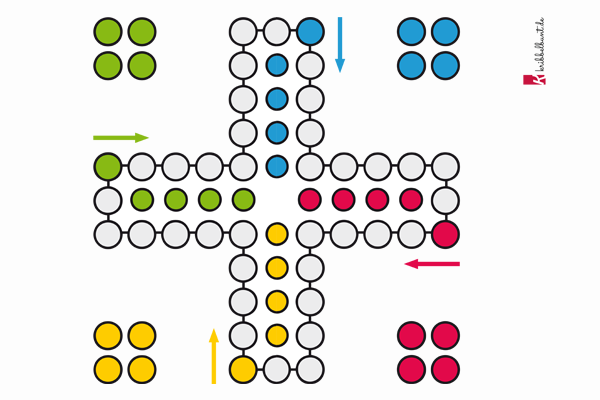
\includegraphics[width=0.31\textwidth]{mensch-aergere-dich-nicht-spielfeld}
	\centering
	\caption{Spielbrett}
\end{wrapfigure}
\begin{enumerate}
	
	\item [$\bullet$] Bei einer gewürfelten Sechs darf erneut gewürfelt werden.
	\item [$\bullet$]Bei einer Sechs wird falls möglich eine eigene Figur auf das Feld A der eigenen Farbe gestellt.
	\item [$\bullet$] Eine Gegnerische Figur die das Zielfeld besetzt wird beim betreten geschlagen (zurück auf eines der B Felder).
	\item [$\bullet$] Die vorderste Figur wird immer als erstes versucht zu bewegen (Abweichung von den Offiziellen Regel)
	\item [$\bullet$] Die Zielfelder [a, b, c, d] müssen genau erreicht werden. Es dürfen keine \glqq Augenzahlen \grqq verfallen
	\item [$\bullet$] Kann die vorderste Figur nicht bewegt werden, wird so lange die nächste weiteste Figur versucht zu bewegen.
	\item [$\bullet$] Kann keine der Figuren auf der \glqq Laufbahn \grqq bewegt werden, verfällt der Zug.
	\item [$\bullet$] Felder auf denen eine eigene Figur steht können nicht betreten werden. Auf den Zielfeldern dürfen eigene Figuren nicht übersprungen werden.
	\item [$\bullet$] Die Spieler führen ihre Züge immer im wechsel aus.
\end{enumerate}


\section{Umsetzung}
%Hier wird kurz erläutert, wie die Lösungsidee im Programm tatsächlich umgesetzt wurde. Hier können auch Implementierungsdetails erwähnt werden.
Die Lösungsidee wird in Python implementiert. Die Python Imaging Library (PIL) stellt viele Funktionen zur Bildverar- beitung zur Verfügung. Damit funktionieren das Öffnen und 
Speichern des Bildes und der Zugriff auf die Pixeldaten sehr einfach. Wir importieren dazu das Modul Image der PIL. Mithilfe zweier ineinander geschachtelter For-Schleifen 
werden alle Pixel einzeln betrachtet. Immer wenn ein Pixel die gleiche Farbe hat wie eines seiner Nachbarpixel, färben wir beide Pixel weiß. Da bei dieser Aufgabe alle Pixel weiß gefärbt werden sollen, die zu einem Rhinozelfant gehören könnten, müssen wir aufpassen, dass wir nicht direkt ein Pixel im Bild weiß färben, wenn wir sehen, dass es einen gleichfarbigen Nachbarn 
gibt. Sonst kann es passieren, dass wir bei den anderen benachbarten Pixeln nicht mehr wissen, welche Farbe das aktuelle Pixel ursprünglich hatte. Dieses Problem wird 
gelöst, indem nicht die Pixel im Originalbild weiß gefärbt werden, sondern in einer Kopie des Bildes ('ausgabebild'). Dadurch können wir im Originalbild immer alle Pixel in ihrer 
ursprünglichen Farbe vergleichen. Zu guter Letzt wird das Ausgabebild wieder in eine Datei 
gespeichert. 
\section{Beispiele}
%Genügend Beispiele einbinden! Die Beispiele von der BwInf-Webseite sollten hier diskutiert werden, aber auch eigene Beispiele sind sehr gut – besonders wenn sie Spezialfälle abdecken. Aber bitte nicht 30 Seiten Programmausgabe hier einfügen!
Wir rufen das Programm für zwei der Beispieldateien auf und zeigen jeweils das resultierende Bild in verkleinerter Darstellung: 
\section{Quellcode}
%Unwichtige Teile des Programms sollen hier nicht abgedruckt werden. Dieser Teil sollte nicht mehr als 2–3 Seiten umfassen, maximal 10.
Beispiel-Code:
\begin{lstlisting}
static void Main(string[] args)
        {
//test Comment!
            List<Player> players = SetPlayers(args);
            List<MatchUps> matchups = CreateMatchups(players);
            List<GameResults> gameresults = PlayGames(matchups);
            RankPlayers(gameresults);
	 Console.WriteLine("Test string");
            
        }
\end{lstlisting}
Program.cs:
\lstinputlisting{DiceCompare/Program.cs}

\end{document}
